\documentclass{beamer}
\mode<presentation>
{
	\usetheme{Frankfurt}      % or try Darmstadt, Madrid, Warsaw, ...
	\usecolortheme{beaver} % or try albatross, beaver, crane, ...
	\usefonttheme{default}  % or try serif, structurebold, ...
	\setbeamertemplate{navigation symbols}{}
	\setbeamertemplate{caption}[numbered]
} 

\usepackage[utf8]{inputenc}
\usepackage[french]{babel}
\usepackage{graphicx}
\usepackage{amssymb}
\usepackage{amsmath}
\usepackage{amsthm}
\usepackage{float}
\usepackage{amsmath}
\usepackage{amssymb}
\usepackage{mathrsfs}
\usepackage{hyperref}
\usepackage{graphicx}
\usepackage{appendix}
\usepackage{hyperref}
\usepackage{subcaption}
\usepackage{setspace}
\usepackage[intoc]{nomencl}
%\usepackage{algorithm}
%\usepackage{listing}
\usepackage{verbatim}
\usepackage{fontawesome}
%Statistics for High Dimensional Data
  \title{Soutenance projet de troisième année : \\
  Algorithme d'apprentissage en chimie quantique et application au screening (sélection) de cellules photovoltaïques}
  \author{Etudiant : Pierre Gauthier\institute{École Mines Nancy}\\
  Tuteurs : Jérémie Unterberg, Marianne Clausel, Dario Rocca}
  \date{5 Février 2019}

% définition de mes fonctions
\addtobeamertemplate{footline}{\hspace{0.5cm} \normalsize \insertframenumber/\inserttotalframenumber \hspace{0.5cm} \small Pierre Gauthier Soutenance projet-3A}
\normalsize
\begin{document}

  \begin{frame}
  	
  	
	\begin{figure}[!h]
	\centering	
		\begin{subfigure}[b]{0.3\textwidth}
		\includegraphics[height = 1cm, keepaspectratio]{graphes/mines_nancy.png}
		\end{subfigure}
		\begin{subfigure}[b]{0.3\textwidth}
		\includegraphics[height = 1cm, keepaspectratio]{graphes/elie_cartan.png}
		\end{subfigure}
		\begin{subfigure}[b]{0.3\textwidth}
		\includegraphics[height = 1cm, keepaspectratio]{graphes/univ_lorraine.png}
	\end{subfigure}
	\end{figure}
	
  \titlepage
  \end{frame}

 

%%%%%%%%%%%%%%%%%%%%%%%%%%%%%%%%%%%%%%%%%%%%%%%%%%%%%%%%%%%%%%%%%%%
\begin{frame}{Introduction}
\begin{itemize}
\item[$\bullet$] Travail sur la publication de Mathias Rupp \textit{Machine Learning for Quantum Mechanics in a Nutshell},  s'inscrit dans le \textit{Harvard Clean Energie Project}
\item[$\bullet$]  Couplage Physique Quantique / Apprentissage automatique
\end{itemize}
\begin{center}
\begin{figure}[!h]

\includegraphics[height = 5cm, keepaspectratio]{graphes/harvard.png}
		\end{figure}
\end{center}
\end{frame}
\begin{frame}
   \tableofcontents
\end{frame}
\section{Description des données}
\begin{frame}{Description des données}
\begin{itemize}
\item[$\bullet$] Dataset de molécules en .xyz :
\end{itemize}
\begin{tabular}{ l c c c }
   Nombre d'atome &  & & \quad\\
   numéro de la molécule &\quad énergie d'atomisation &\quad &\\
   atome 1 & x(1) & y(1) & \quad z(1) \\
   atome 2 & x(2) & y(2) & \quad z(2) \\
   . & . & . & \quad . \\
   . & . & . & \quad . \\
   . & . & . & \quad . \\
   atome n & x(n) & y(n) &\quad  z(n) \\
 \end{tabular}
\end{frame}
\begin{frame}{Description des données}
\begin{itemize}
\item[$\bullet$] Utilisation des Matrices de Coulomb (Z numéro atomique):
\[
M_{ij} = 
	\left\{
	\begin{array}{ccc}		
	\begin{aligned}
		& 0.5 Z_{i}^{2.4} \quad &i=j\\
		& \frac{Z_i Z_j}{||R_i - R_j||_{2}} \quad &i\neq j
	\end{aligned}
\end{array}
	\right.
\]
\item[$\bullet$] Matrice sysmétrique, de taille $23\times23$ $\rightarrow$ stockage dans vecteur taille $\frac{23\times(23+1)}{2} = 276$.
\item[$\bullet$] La matrice varie avec permutation des atomes $\rightarrow$ Tri des lignes par norme décroissante
\end{itemize}
\end{frame}
\begin{frame}{Description des données}
Exemple simple de matrice Coulombs pour C$-$H et H$-$C$-$H:
\\
\begin{tabular}{ l | c c c c }
	 & C 	& H 	&   &		\\
	 \hline
   C & a$_1$ & b$_1$ &  0 & 0   \\
   H & b$_1$ & a$_2$ &	0 & 0	\\
    & 0 & 0 & 0 & 0	 \\
   & 0 & 0 & 0 & 0 \\
    \end{tabular} $\rightarrow$ ( a$_1$, b$_1$, 0, 0, a$_2$, 0, 0, 0, 0, 0)
  \newline
\begin{tabular}{ l | c c c c }
	 & C 	& H 	& H  &		\\
	 \hline
   C & a$_1$ & b$_1$ &  c$_1$ & 0   \\
   H & b$_1$ & a$_2$ &	c$_2$ & 0	\\
   H & c$_1$ & c$_2$ &	a$_3$ & 0	\\
   & 0 & 0 & 0 & 0 \\
    \end{tabular}  $\rightarrow$ ( a$_1$, b$_1$, c$_1$, 0, b$_1$, a$_2$, c$_2$,0 ,a$_3$, 0)
\end{frame}
\section{Outils d'apprentissage automatique}
\subsection{Support Vector Machines methods (SVM)}
\begin{frame}{Support Vector Machines methods (SVM)}
Nous allons commencer par présenter le problème de classification avant la régression
\begin{figure}[!h]
	\begin{center}
	\centering	
	%\begin{subfigure}[b]{0.3\textwidth}
		\includegraphics[height = 3.5cm, keepaspectratio]{graphes/SVM_donnee.png}
		\includegraphics[height = 3.5cm, keepaspectratio]{graphes/SVM_separee.png}
					%\end{subfigure}
	\end{center}
\end{figure}
\end{frame}
\begin{frame}{Support Vector Machines methods (SVM)}
 Hyperplan de séparation 
\[
H = \{x | w^T x + b =0\} \quad
\text{Marge}(H) = \text{min}_{x_{i}}\ d(x_i,\ H)
\]

\begin{figure}[!h]
	\begin{center}
	\centering	
	%\begin{subfigure}[b]{0.3\textwidth}
		\includegraphics[height =5cm, keepaspectratio]{graphes/svm05.png}
	\end{center}
\end{figure}
\end{frame}
\begin{frame}{Support Vector Machines methods (SVM)}
\begin{figure}[!h]
	\begin{center}
	\centering	
	%\begin{subfigure}[b]{0.3\textwidth}
		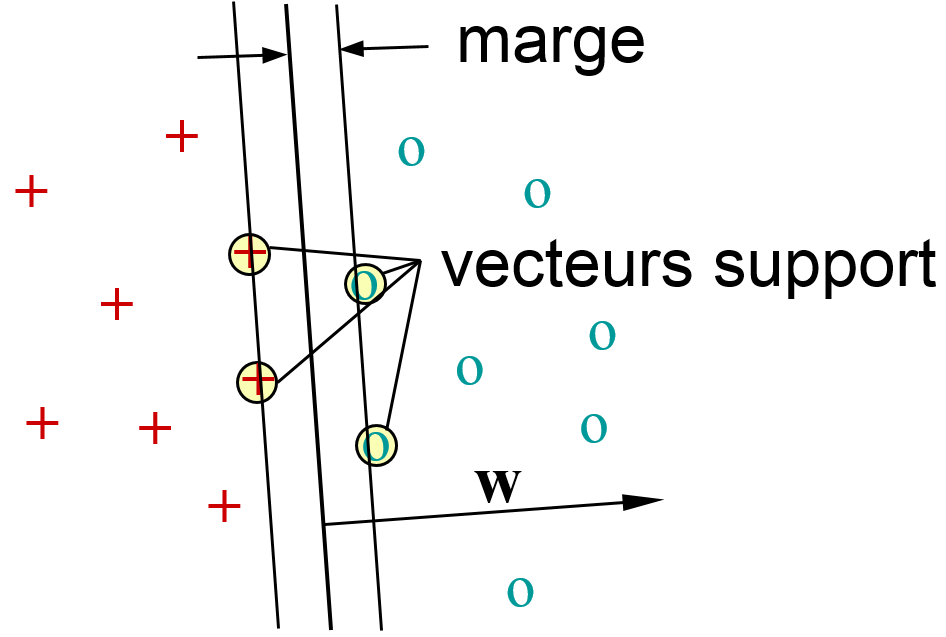
\includegraphics[height =3cm, keepaspectratio]{graphes/svm07.png}
			%\end{subfigure}
	\end{center}
\end{figure}
\[ 
2 \times \text{Marge} = 2 \times d(x,\ H) = \frac{|w^T x_{vs} + b|}{||w||}
\]
\[|w^T x_{vs} + b| = 1 \quad \rightarrow \quad \text{Marge} = \frac{2}{||w||} \]
\end{frame}
\begin{frame}{Support Vector Machines methods (SVM)}
On en arrive au problème de minimisation suivant : 
\[
	\left\{
	\begin{array}{ccc}		
	\begin{aligned}
		&\text{arg}\ \text{min}_{w,b}\ \frac{1}{2}||w||^{2} \\
		&\forall \ 1 \leqslant i \leqslant N,\ y_i (w \cdot x_i + b)\geqslant 1
	\end{aligned}
\end{array}
	\right.
% − \sum{ \lambda_{i} (y_{i} (w \cdot x_i + b)−1)}
\]
On formule le problème dual en introduisant le Laplacien :
\[
\left\{
\begin{array}{lll}
	\text{max}\ L(\lambda) = \sum_{i}{\lambda_{i}} - \frac{1}{2} \sum_{i}{\sum_{j}	{\lambda_{i} \lambda_{j} y_i y_j x_i \cdot x_j}} \\
 \lambda_i \geqslant 0 \\
 \sum_{i}\lambda_i y_i = 0 
\end{array}
\right.
\]
\[
	f^* (x) = \sum_{i=1}^n {\lambda^*_i y_i x^T_i x + b^*}
\]
\end{frame}
\subsection{Astuce du noyau}
\begin{frame}{Astuce du noyau}
Augmentation de la dimension de l'espace pour rendre les données linéairement séparables
\begin{figure}[!h]
	\begin{center}
	%\begin{subfigure}[b]{0.3\textwidth}
		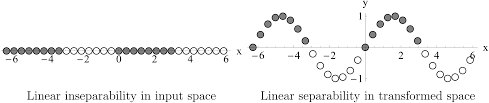
\includegraphics[height = 2cm, keepaspectratio]{graphes/separation.png}
			%\end{subfigure}
	\end{center}
\end{figure}
\end{frame}
\begin{frame}{Astuce du noyau}
\[
	f (x) = \sum_{i=1}^n {\lambda_i y_i x^T_i x + b} \rightarrow 
\sum_{i=1}^n {\lambda_i y_i K(x_i,x) + b}
\]
Si K doit vérifier les conditions :
\begin{itemize}
\item[$\bullet$]  $K$ est continue symétrique 
\item[$\bullet$]  $K(x_i,x_j)_{\ 1 \leqslant i,j \leqslant N}$ est une matrice définie positive
\end{itemize}
 Alors il existe $\phi :\xi \rightarrow H$ telle que $K(x,y) = \langle\phi(x),\phi(y)\rangle$.
\end{frame}
\subsection{Ridge Regression}
\begin{frame}{Ridge Régression}
On ajoute un terme de pénalisation $|.|_2^2$ au problème de régression classique
\[
\underset{w \in \mathbb{R}^{n}}{\text{arg min}}\sum{(f(x_i) - y_i)^{2}} \quad \rightarrow \quad \underset{w \in \mathbb{R}^{n}}{\text{arg min}}\sum{(f(x_i) - y_i)^{2}} +  \lambda ||w||_2^{2}
\]
\[
w = (X^T X)^{-1} X^T y\quad \rightarrow \quad w^{ridge} = (X^T X + \lambda I)^{-1} X^T y
\]
\end{frame}
\begin{frame}{Ridge Régression}

\begin{figure}[!h]
	\begin{center}
	\centering	
	%\begin{subfigure}[b]{0.3\textwidth}
		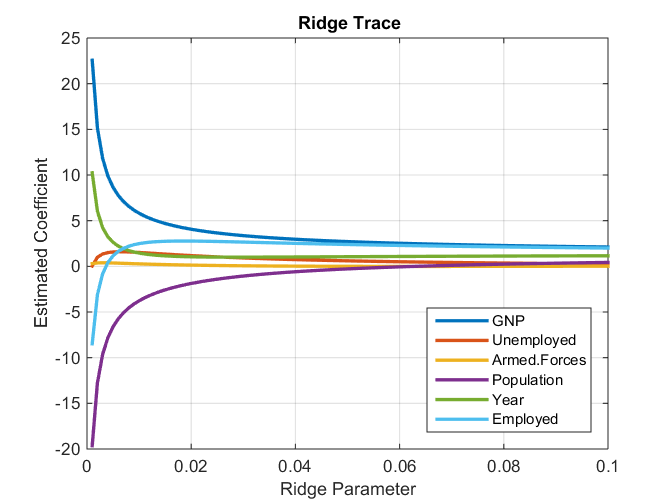
\includegraphics[height =4cm, keepaspectratio]{graphes/ridge.png}
			%\end{subfigure}
		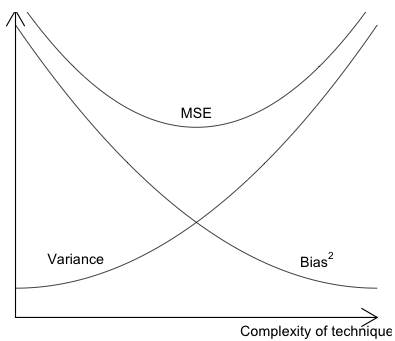
\includegraphics[height =4cm, keepaspectratio]{graphes/ridge_trade.png}
			%\end{subfigure}
	\end{center}
\end{figure}
\end{frame}
\begin{frame}{Ridge Régression}
Applications aux méthodes à noyaux avec $f(x) = \sum_{i = 1}^{n}{\alpha_i \text{K}(x_i , x)}$
\[
\begin{aligned}
&\underset{\alpha \in \mathbb{R}^{n}}{\text{arg min}}\sum{(f(x_i) - y_i)^{2}} +  \lambda ||f||_H^{2} \\
\Leftrightarrow
& \ \underset{\alpha \in \mathbb{R}^{n}}{\text{arg min}}<K \alpha - y , K 	\alpha -y > + \lambda \alpha^{T} K \alpha \\
\Rightarrow \ & \alpha	=(K + \lambda I)^{-1}y
\end{aligned}
\]
Avec $K \in \mathbb{R}^{n \times n} \text{ est la matrice du 			noyau} \quad K_{i,j} = K(x_i, x_j)$
\end{frame}
\section{Expérimentations}
\subsection{Base d'entrainement et de Test du modèle}
\begin{frame}{Base d'entrainement et de Test du modèle}
On séparer le dataset d'environ 7000 molécules en \newline
\begin{itemize}
\item[$\bullet$] un set d'entrainement de 900 molécules $\rightarrow$ recherche des hyperparamètres ($\lambda$, paramètres des noyaux)
\newline
\item[$\bullet$] un hold-out set de 100 molécules pour vérifier qu'il n'y a pas de sur-apprentissage sur le set d'entrainement
\newline
\item[$\bullet$] Un set de prédiction avec reste des molécules.
\end{itemize}
\end{frame}
\subsection{Fonctions d'erreurs utilisées}
\begin{frame}{Fonctions d'erreurs utilisées}
\begin{itemize}
\item[$\bullet$] $\text{RMSE} = \sqrt{\frac{1}{n}\sum_{i=}^n {(y_i - f(x_i))^2}}$
\newline
\item[$\bullet$]$\text{MAE} = \frac{1}{n}\sum_{i=}^n {|y_i - f(x_i)|}$
\newline
\item[$\bullet$]$(1 - R^2) \sum_{i=1}^n {(\overline{y} - y_i)^2} = \sum_{i=}^n {(y_i - f(x_i))^2} $
\end{itemize}
\end{frame}
\subsection{Recherche hyparamètres optimaux}
\begin{frame}{Recherche hyparamètres optimaux}
Présentation des noyaux utilisés :\\
\textbf{Noyau Gaussien}
\[ 
	K(x,z) = \exp{- \frac{||x-z||_{2}^2}{2\sigma^2}}  = \exp{- \gamma ||x-z||_{2}^2}
\]
\textbf{Noyau Laplacien}
\[ 
	K(x,z) = \exp{- \frac{||x-z||_{1}}{\sigma}} =  \exp{- \gamma ||x-z||_{1}}
\]
\end{frame}
\begin{frame}{Résultats noyau gaussien}
\begin{figure}[!h]	
		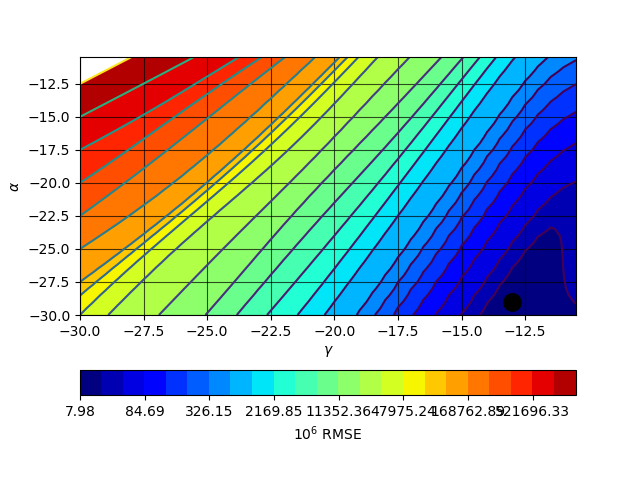
\includegraphics[height = 3.9cm, keepaspectratio]{graphes/resultat_RBF_RMSE.png}
		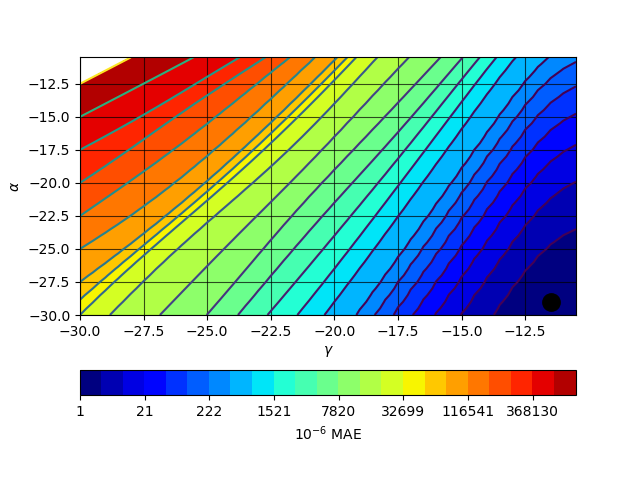
\includegraphics[height = 3.9cm, keepaspectratio]{graphes/resultat_RBF_MAE.png}
		\end{figure}
\end{frame}
\begin{frame}{Résultats noyau laplacien}
\begin{figure}[!h]	
		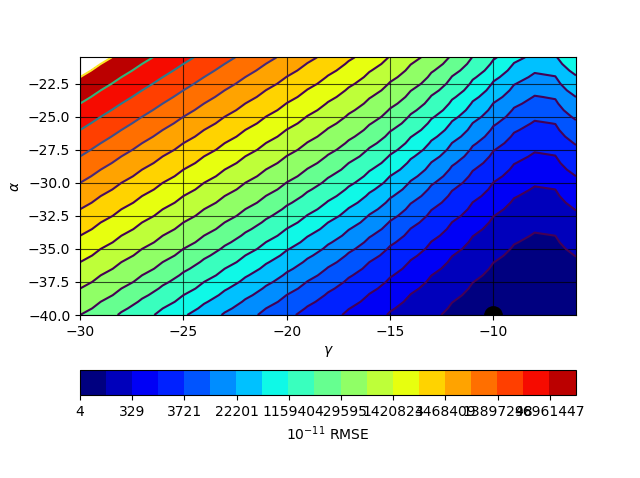
\includegraphics[height = 3.9cm, keepaspectratio]{graphes/resultat_Lapla_RMSE.png}
		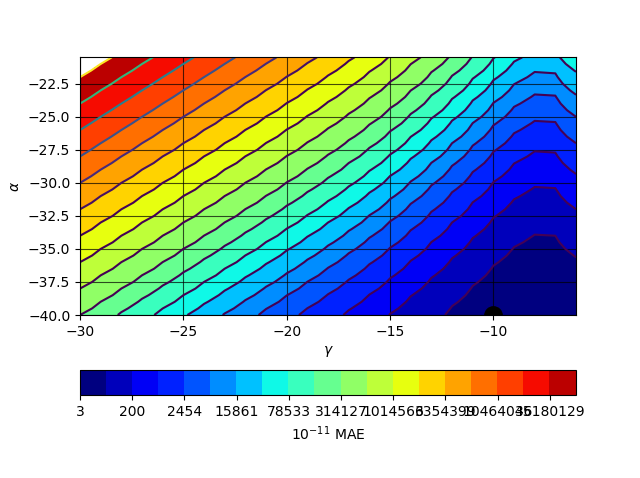
\includegraphics[height = 3.9cm, keepaspectratio]{graphes/resultat_Lapla_MAE.png}
		\end{figure}
\end{frame}
\begin{frame}{Recherche hyparamètres optimaux}
\begin{center}
\begin{tabular}{ l| c c c }

   Erreur utilisée  & RMSE & MAE & R$^2$ \\
   \hline
   KRR avec noyau gaussien & 9.6371 & 7.6962 & 0.9977\\
   KRR avec noyau laplacien  & 5.4019 & 3.4555 & 0.9993\\
  \end{tabular}
  \end{center}
\end{frame}
\section{Perspectives}
\begin{frame}{Perspectives}
\begin{itemize}
\item[$\bullet$] Utilisation d'autres modèle comme Random Forest
\newline
\item[$\bullet$]Utilisation d'autres descripteurs que les matrices de Coulomb
\end{itemize}
\end{frame}
\section{Conclusion}

\begin{frame}{Conclusion}
\begin{itemize}
\item[$\bullet$] Un projet efficient pour développer ces compétences en machine learning.
\newline
\item[$\bullet$] Nous avons reproduis l'article scientifique
\item[$\bullet$] Nous ne sommes pas allé plus loin...
\end{itemize}
\end{frame}

\begin{frame}
\begin{center}
\textbf{Merci de votre attention}
\end{center}
\end{frame}


\end{document}
